\documentclass[11pt]{article}

% ---- fonts: Latin Modern (bundled with tectonic), clean academic look ----
\usepackage{lmodern}
\usepackage[T1]{fontenc}

% ---- layout ----
\usepackage[letterpaper,margin=1.1in]{geometry}
\usepackage{microtype}
\usepackage{parskip}
\usepackage[dvipsnames]{xcolor}
\usepackage{booktabs}
\usepackage{tabularx}
\usepackage{array}
\usepackage{titlesec}
\usepackage{enumitem}
\usepackage{graphicx}
\usepackage{caption}
\usepackage{tikz}
\usetikzlibrary{positioning,arrows.meta,calc,fit,backgrounds,shapes.geometric}
\usepackage[most]{tcolorbox}
\usepackage[htt]{hyphenat}
\usepackage{hyperref}

\setlength{\emergencystretch}{2em}

% ---- palette ----
\definecolor{ankrblue}{HTML}{2457D6}
\definecolor{ankrink}{HTML}{15181E}
\definecolor{ankrpanel}{HTML}{F3F6FC}
\definecolor{ankrhilite}{HTML}{E4ECFC}
\definecolor{ankrline}{HTML}{C6D1E6}
\definecolor{ankrgrey}{HTML}{5B6472}
\definecolor{ankrred}{HTML}{C0392B}
\definecolor{ankrgreen}{HTML}{1E7A46}

\hypersetup{
  colorlinks=true, linkcolor=ankrblue, urlcolor=ankrblue, citecolor=ankrblue,
  pdftitle={Token Optimized RPC: Reading a Blockchain Without Drowning an Agent in Tokens},
  pdfauthor={Mike Kondratev, Alexander Kolesov, Roman Fasakhov, Stanley Wu (Web3 Technologies, Inc., dba Ankr)}
}

\captionsetup{font=small, labelfont={bf,sf,color=ankrblue}, labelsep=period, textfont=it}

% ---- section styling ----
\titleformat{\section}{\sffamily\large\bfseries\color{ankrblue}}{\thesection.}{0.6em}{}
\titlespacing*{\section}{0pt}{1.5em}{0.4em}

% ---- callout boxes ----
\newtcolorbox{onepara}{enhanced, breakable, colback=ankrpanel, colframe=ankrblue,
  boxrule=0pt, leftrule=3pt, arc=1pt, left=10pt, right=10pt, top=8pt, bottom=8pt,
  fonttitle=\sffamily\bfseries\color{ankrblue}, title={In one paragraph}}

\newtcolorbox{guaranteebox}{enhanced, breakable, colback=ankrhilite, colframe=ankrblue,
  boxrule=0.6pt, arc=2pt, left=10pt, right=10pt, top=8pt, bottom=8pt,
  coltitle=white, colbacktitle=ankrblue, fonttitle=\sffamily\bfseries,
  title={The correctness contract}}

\newtcolorbox{infobox}[1]{enhanced, breakable, colback=ankrpanel, colframe=ankrline,
  boxrule=0.6pt, arc=2pt, left=10pt, right=10pt, top=8pt, bottom=8pt,
  fonttitle=\sffamily\bfseries\color{ankrink}, title={#1}}

\newtcolorbox{codebox}[1]{enhanced, breakable, colback=ankrpanel, colframe=ankrline,
  boxrule=0.6pt, arc=2pt, left=12pt, right=12pt, top=8pt, bottom=8pt,
  fontupper=\ttfamily\scriptsize, coltitle=ankrink,
  fonttitle=\sffamily\bfseries\footnotesize, title={#1}}

\newcommand{\code}[1]{\texttt{#1}}

\begin{document}

% ============ TITLE PAGE ============
\begin{titlepage}
\centering
\vspace*{1.1in}
{\sffamily\small\color{ankrgrey} WEB3 TECHNOLOGIES, INC. \enskip(DBA ANKR)}\\[2.4em]
{\sffamily\bfseries\Huge\color{ankrink} Token Optimized RPC}\\[0.6em]
{\sffamily\LARGE\color{ankrblue} Reading a Blockchain Without Drowning an Agent in Tokens}\\[1.5em]
{\color{ankrline}\rule{0.45\textwidth}{1pt}}\\[1.5em]
{\sffamily\normalsize\color{ankrgrey} Mike Kondratev \textbullet\ Alexander Kolesov \textbullet\ Roman Fasakhov \textbullet\ Stanley Wu}\\[0.8em]
{\sffamily\normalsize\color{ankrgrey} Whitepaper draft 0.9, describing TORPC/TOEVM spec v1 \textbullet\ July 2026}\\[3.2em]
{\itshape\large The chain answers in bytes. The agent pays in tokens.\\[0.2em] TORPC stops it paying for noise.}
\vfill
{\sffamily\footnotesize\color{ankrgrey} spec \code{github.com/w3tech/torpc} (CC0-1.0) \enskip\textbullet\enskip code \code{github.com/w3tech/torpc-js} (Apache-2.0)}
\end{titlepage}

% ============ ON-RAMP + ABSTRACT + TOC ============
\begin{onepara}
When an AI agent reads a blockchain through a JSON-RPC endpoint, it pays for every byte the node returns: hex strings a model must decode in its head, a \code{logsBloom} filter it never reads, repeated field names, structural punctuation. Those bytes become input tokens on every call, and for a receipt-heavy workload they dominate the bill and crowd the context window. TORPC is a token-optimized rendering of the same data: the node's response is decoded, renamed, and stripped of what an agent cannot use, negotiated by a single HTTP header. Nothing is invented, and the raw response is one re-query away. It is not a new API and needs no client schema. On a measured production run the semantic tier cuts tokens per response by 48\% overall and up to two-thirds on receipts, and a three-model accuracy benchmark shows the model answers \emph{better} from the smaller payload than from raw JSON-RPC. The operator does the decoding once, server-side, so every agent downstream stops paying for it.
\end{onepara}

\begin{abstract}
\noindent An AI agent that reads a blockchain through a hosted RPC endpoint pays a tax it never chose. JSON-RPC was designed for programs, not language models: numbers arrive as hex strings the model must convert, addresses in mixed case, event logs as undecoded topic-and-data blobs, a 256-byte \code{logsBloom} on every receipt, and field names repeated for every element of every array. A program ignores the cost; a model pays for all of it in input tokens, on every call, and a single receipt-heavy read can cost a thousand tokens of which a fraction is signal.

\noindent TORPC removes that tax without changing the API. A client opts in with one request header; the endpoint returns the same data re-rendered for a model: hex converted to decimal, addresses checksummed, logs ABI-decoded and collapsed, dead fields dropped by published per-method lists, keys normalized. Nothing is invented: the tier-1 transforms on carried fields are mechanically reversible, the enumerated service fields are dropped by policy, and they are recovered by re-issuing the request without the opt-in header against the same block. The transform is tiered (mechanical or fully decoded), deterministic (identical input yields identical output, so prompt caches hit), and conservative by rule: unenumerated fields pass through verbatim, failed transforms fall back to the verbatim field, and anything the server cannot decode is kept raw and flagged rather than dropped or guessed. In a measured run against the live production proxy the covered read methods shrink by 35\% at the mechanical tier and 48\% at the semantic tier, token-weighted, with receipts at $-64.5\%$ and calldata-bearing transactions at $-69.0\%$; on a three-model accuracy suite the semantic tier \emph{raises} retrieval accuracy on every model tested - all three land at 91-93\%, against 69-82\% from raw - while cutting the suite's corpus by 45\% of its tokens. The format is small by design - one header pair plus public per-method mapping rules, EVM first with the pattern reserved for other chains - published CC0-1.0 with Apache-2.0 reference tooling, and deliberately aligned with existing agent-API standards rather than built as a proprietary stack.
\end{abstract}

{\hypersetup{linkcolor=ankrink}\tableofcontents}
\newpage

% ============ 1 ============
\section{The tax you didn't ask for}

A blockchain node speaks JSON-RPC, a format designed in 2010 for programs talking to programs. A program does not care that a block number arrives as \code{"0x14913f6"}, that a receipt carries a 256-byte bloom filter it will never inspect, or that a hundred-element log array repeats the same eight field names a hundred times. It parses the bytes, pulls the fields it wants, and discards the rest at no cost.

A language model is not a program, and it pays differently. Every byte in the response becomes an input token the moment the agent puts it in context. The hex it has to convert in its head, the checksummed and non-checksummed addresses it has to reconcile, the \code{logsBloom} that means nothing to it, the structural braces and repeated keys of pretty-printed JSON: all of it is billed, on every call, at the model's per-token price. And it competes for the context window, so a few receipt reads can crowd out the reasoning the agent was supposed to do.

The numbers are not marginal. Even the receipt of a plain, single-log USDC transfer weighs about 700 tokens, roughly 75 of them the bloom filter alone; a receipt for a busy contract call runs to thousands, most of it structure and undecoded blobs rather than the handful of facts the agent needs: who called what, did it succeed, what did it transfer, what did it cost. Multiply by the call volume of an analytics pipeline, a wallet copilot, or a trading agent, and the token cost of \emph{reading} the chain becomes a real line item, sometimes larger than the model reasoning it feeds.

The pain is not specific to blockchains: the MCP issue tracker carries a proposal literally titled ``Mitigating Token Bloat'' and standing requests for hard response-size limits \cite{mcpbloat, mcpsize}, and a general-purpose compression layer for agent tool output collected tens of thousands of GitHub stars within months of appearing (as of July 2026) \cite{headroom}. What is specific to blockchains is that the data is unusually hostile to a model (pervasive hex, undecoded ABI, filters and blooms) and unusually mechanical to fix, because the node already knows the ABI and the types. The decoding a model would do, token by token, in its head, the server can do once, for everyone, before the bytes are ever billed.

\begin{figure}[h]
\centering
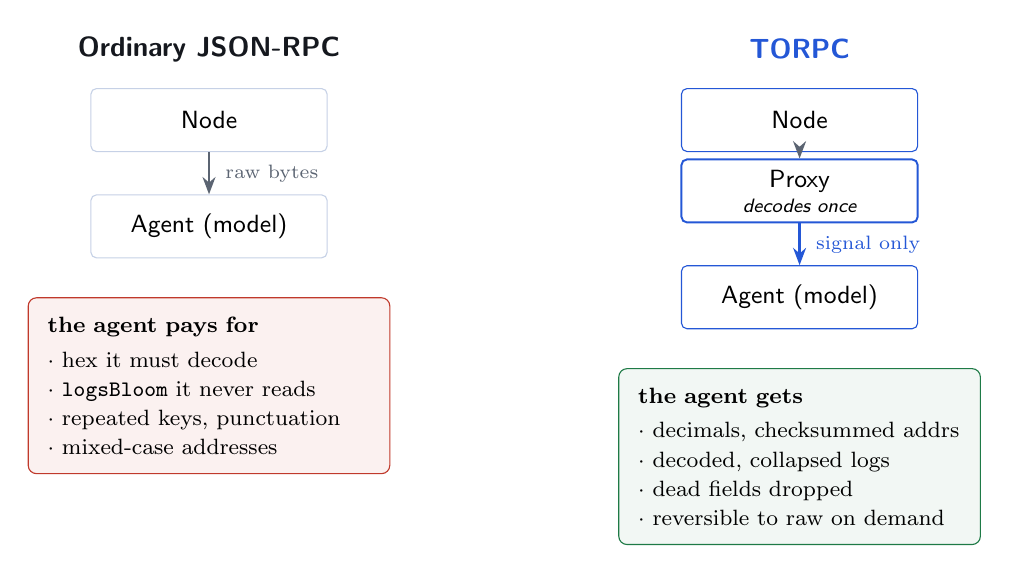
\begin{tikzpicture}[font=\sffamily\small,
  bx/.style={draw=ankrline, rounded corners=2pt, fill=white, align=center, minimum width=3.0cm, minimum height=0.8cm, inner sep=3pt},
  tset/.style={rounded corners=3pt, align=left, inner sep=7pt, text width=4.1cm, font=\footnotesize},
  flow/.style={-{Stealth[length=2.2mm]}, draw=ankrgrey, thick}]
% ===== left: ordinary RPC =====
\node[font=\sffamily\bfseries\color{ankrink}] at (2.9,5.15) {Ordinary JSON-RPC};
\node[bx] (n1) at (2.9,4.25) {Node};
\node[bx] (a1) at (2.9,2.9) {Agent (model)};
\draw[flow] (n1) -- node[right, font=\scriptsize\color{ankrgrey}]{\;raw bytes} (a1);
\node[tset, draw=ankrred, fill=ankrred!7, anchor=north] (yt1) at (2.9,2.0) {\textbf{the agent pays for}\\[3pt]$\cdot$ hex it must decode\\[1pt]$\cdot$ \code{logsBloom} it never reads\\[1pt]$\cdot$ repeated keys, punctuation\\[1pt]$\cdot$ mixed-case addresses};
% ===== right: TORPC =====
\node[font=\sffamily\bfseries\color{ankrblue}] at (10.4,5.15) {TORPC};
\node[bx, draw=ankrblue] (n2) at (10.4,4.25) {Node};
\node[bx, draw=ankrblue, line width=0.7pt] (p2) at (10.4,3.35) {Proxy\\[-2pt]{\scriptsize\itshape decodes once}};
\node[bx, draw=ankrblue] (a2) at (10.4,2.0) {Agent (model)};
\draw[flow] (n2) -- (p2);
\draw[flow, draw=ankrblue] (p2) -- node[right, font=\scriptsize\color{ankrblue}]{\;signal only} (a2);
\node[tset, draw=ankrgreen, fill=ankrgreen!6, anchor=north] (yt2) at (10.4,1.1) {\textbf{the agent gets}\\[3pt]$\cdot$ decimals, checksummed addrs\\[1pt]$\cdot$ decoded, collapsed logs\\[1pt]$\cdot$ dead fields dropped\\[1pt]$\cdot$ reversible to raw on demand};
\end{tikzpicture}
\caption{The work does not disappear, it moves. Ordinary JSON-RPC ships the node's raw bytes and the model pays, in tokens, to decode them on every call. TORPC does the decoding once in the proxy, server-side, so the agent receives only what it can use and every agent downstream stops paying for the same conversion.}
\end{figure}

% ============ 2 ============
\section{The idea}

The mechanism is small enough to state in one sentence: let a client ask, with one HTTP header, for the node's response re-rendered for a language model, and have the endpoint return the same facts decoded, normalized, and stripped of what a model cannot use, with the standard raw response one re-query away.

Three properties make it safe to turn on by default. First, it is \textbf{opt-in and recoverable}: an unmodified client sees standard JSON-RPC; the tier-1 transforms on carried fields are mechanically reversible; and the enumerated service fields the transform drops by policy are recovered by re-issuing the request without the opt-in header, against the same block. That re-query is content negotiation against a live node rather than a retention contract, so archival availability is not guaranteed and a client that needs reproducibility pins a block. Second, it is \textbf{tiered and best-effort}: the client names the \emph{highest} tier it will accept, from a mechanical pass (hex to decimal, dead-weight drops) to a full semantic decode (ABI-resolved logs and calldata), and the server serves the highest tier it can honor for that method and that payload - never more. Third, it is \textbf{deterministic}: at a given tier, the same raw response renders to the same bytes from a given server (and to the same fields and values from any conforming one - \S5), so response-level caches (HTTP, client-side memoization) key on stable content, and repeated identical reads stay prefix-cacheable on the model side.

\textbf{Where this matters most.} The token you save scales with how often you read and how noisy the read is. A high-volume agent living on receipts, logs, and traces (analytics, indexing, wallet copilots, trading infrastructure with an LLM in the loop) is the case for it; there, half the tokens is half the bill and twice the headroom in context. For an occasional, small read, plain RPC is fine. TORPC is for the workloads where reading the chain is a cost center, not an afterthought.

\textbf{Why the server does it - and why it doesn't have to.} The mechanical tier is a pure function of the raw response, so nothing stops a client from running the same transform locally; the reference mapper ships as a package in the code repository (\code{@torpc/decoder}, structural only: no ABI, no decoding, and source-only for now rather than on a public registry) precisely so it can, and a local transform earns the identical token saving with no trust placed in the provider. What TORPC standardizes is the \emph{rendering}, not the placement: because the per-method rules are published and deterministic, a local transform and a conforming server produce the same bytes, and the header negotiation is simply the deployment that reaches clients which cannot run a transform at all - a bare \code{curl}, an MCP tool call, a hosted agent runtime with no preprocessing hook. The semantic tier is where the server placement earns its keep: ABI resolution wants a curated, continuously updated signature-and-contract corpus, which is operational data a provider maintains anyway and most clients do not want to host, and running it once on the response path amortizes the decode across every agent downstream instead of re-implementing it in each harness. A client that prefers sovereignty over convenience loses nothing by decoding locally; a client that cannot, opts in with one header.

% ============ 3 ============
\section{What stays the same}

The first question to ask of any transform that rewrites data is what it can lose. For TORPC the answer is the point of the design, so it goes up front. Here is exactly what a TORPC response preserves, and what it deliberately changes.

\textbf{The API does not change.} TORPC is not a new protocol with new methods. It is a rendering of the responses of the JSON-RPC methods that already exist. A client calls \code{eth\_getTransactionReceipt} the way it always did; the only difference is one request header and the shape of the value that comes back. The JSON-RPC~2.0 envelope is preserved verbatim (\code{jsonrpc}, \code{id}, the \code{result}/\code{error} frame), and JSON-RPC \emph{error} responses are never touched at any tier - an \code{error} object comes back exactly as the node produced it, so failure handling looks the way it always did. There is no schema to ship, no SDK required, no new endpoint to learn. A client that does nothing gets ordinary JSON-RPC. The corollary deserves its own sentence: the rendered \code{result} is meant for a model's context, not for typed client libraries - the renames and re-typed values that help a model will break a parser expecting standard field names, so do not enable the opt-in on a transport shared with viem/ethers-style code. Opt in on the path that feeds the model; leave every other connection untouched.

\textbf{Nothing is dropped silently, and nothing is guessed.} Every field of the raw response falls into one of three published classes. It is \emph{carried} - usually re-typed into a form a model reads directly (hex integer to decimal string, address to its EIP-55 form) or renamed to one canonical key. Or it is \emph{redundant within the response} and collapsed: a receipt's logs each repeat the receipt's own block number, block hash, and transaction hash, and TORPC keeps those once at the top level instead of once per log. Or it is \emph{node-internal bookkeeping} - the 256-byte \code{logsBloom} (derivable from the very logs it summarizes), running counters like \code{cumulativeGasUsed}, envelope tags - dropped by an enumerated, published per-method list, never ad hoc. Two hard rules police the boundary. Fields \emph{not} named in a method's ruleset - a chain-specific extension such as Optimism's \code{l1Fee*} or Arbitrum's \code{gasUsedForL1}, or a field added by a post-spec EIP - \textbf{must} pass through verbatim, untransformed. And a transform that fails on a malformed or unexpected field \textbf{must} fall back to the verbatim field rather than drop it, invent a value, or abandon the rest of the response. At the semantic tier, an element the server cannot decode - an event whose ABI it cannot resolve - is kept raw and flagged (\code{\_event\_unknown}, \code{\_function\_unknown}); the spec's normative language is blunt: servers \textbf{must not} invent a decoding. A decoded receipt with fourteen logs where one is unknown returns thirteen decoded and one raw, never thirteen.

\textbf{The raw response is one re-query away.} The escape hatch is HTTP content negotiation, not a retention contract: re-issue the same request, with the same authentication, without the TORPC opt-in, and the endpoint returns the standard JSON-RPC response. Two limits come with that. For snapshot consistency across the two calls a client pins a block number or hash in the underlying call, exactly as it would with any RPC provider - behind a load-balanced endpoint consecutive answers may come from different nodes, and a reorg between the two reads is a property of Ethereum, not of TORPC. And the re-query can only return what the node still serves: archival depth is an operational property of the deployment, not a retention promise attached to the format, so an agent that needs a rendering to stay reproducible pins the block it read.

\begin{infobox}{What changes, and what it costs a reader}
\begin{itemize}[leftmargin=1.4em, itemsep=2pt, topsep=2pt]
\item \textbf{Numerics become decimal strings.} \code{"0x17ee5d9"} $\to$ \code{"25093593"}. A model reads it directly; no in-head hex conversion, and exactness survives any magnitude because the value stays a string. A few enumerated status codes additionally render as words (\code{"0x1"} $\to$ \code{"success"}) - a value map published in the ruleset like any other rule.
\item \textbf{Addresses become EIP-55 checksummed strings} \cite{eip55}. One canonical form, so the model does not reconcile cases.
\item \textbf{Keys are renamed once, per a published per-method map} (\code{transactionHash} $\to$ \code{tx}, \code{effectiveGasPrice} $\to$ \code{gas\_price}), and enumerated dead-field lists drop node bookkeeping (\code{logsBloom}, \code{cumulativeGasUsed}). Never ad hoc: unenumerated fields pass through verbatim.
\item \textbf{Logs and inputs are ABI-decoded} into named events and functions with named arguments. \emph{Caveat:} argument names are derived by the proxy and may differ from the canonical ABI (an ERC-20 \code{transfer} may decode as \code{recipient}/\code{amount} rather than \code{to}/\code{value}); do not assume canonical names.
\end{itemize}
\end{infobox}

% ============ 4 ============
\section{How it works}

Four moving parts: the tier ceiling a client names, the header pair that negotiates it, the server-side transform, and the escape hatch back to raw. Everything happens inside \code{result} on success responses; the envelope and all error responses are out of bounds by rule.

\begin{figure}[h]
\centering
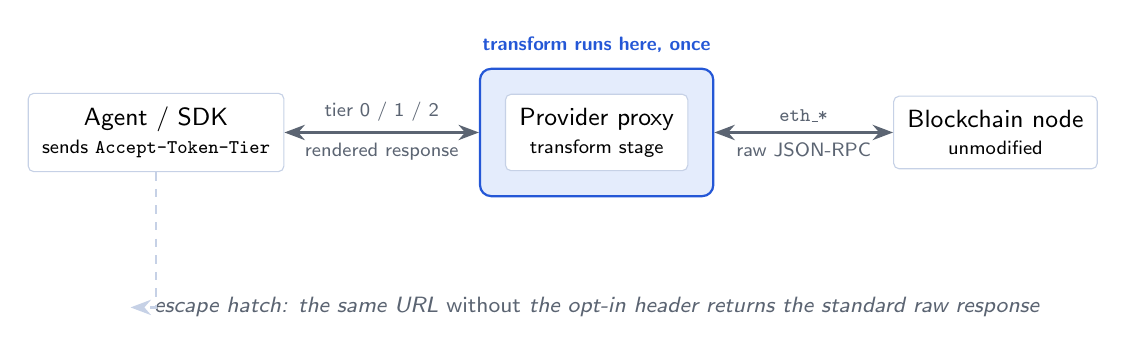
\begin{tikzpicture}[font=\sffamily\small,
  box/.style={draw=ankrline, rounded corners=2pt, fill=white, align=center, inner sep=5pt, minimum height=0.9cm},
  albl/.style={font=\sffamily\scriptsize, text=ankrgrey, inner sep=1.5pt},
  arr/.style={-{Stealth[length=2.6mm]}, draw=ankrgrey, thick},
  bidir/.style={{Stealth[length=2.6mm]}-{Stealth[length=2.6mm]}, draw=ankrgrey, thick}]
\node[box] (client) {Agent / SDK\\[-1pt]\scriptsize sends \code{Accept-Token-Tier}};
\node[box, right=2.8cm of client] (proxy) {Provider proxy\\[-1pt]\scriptsize transform stage};
\node[box, right=2.6cm of proxy] (node) {Blockchain node\\[-1pt]\scriptsize unmodified};
\begin{scope}[on background layer]
  \node[draw=ankrblue, thick, rounded corners=4pt, fill=ankrhilite, fit=(proxy), inner sep=9pt] (encA) {};
\end{scope}
\node[font=\sffamily\bfseries\scriptsize\color{ankrblue}, above=2pt of encA.north] {transform runs here, once};
\draw[bidir] (client) -- node[albl, above=2pt]{tier 0 / 1 / 2} node[albl, below=2pt]{rendered response} (encA);
\draw[bidir] (encA) -- node[albl, above=2pt]{\code{eth\_*}} node[albl, below=2pt]{raw JSON-RPC} (node);
\node[font=\sffamily\itshape\footnotesize\color{ankrgrey}, below=1.15cm of encA.south, anchor=north, align=center] (esc)
  {escape hatch: the same URL \emph{without} the opt-in header returns the standard raw response};
\draw[arr, draw=ankrline, dashed] (client.south) |- ([xshift=-5pt]esc.west);
\end{tikzpicture}
\caption{A client negotiates a tier with one request header; the transform (in Ankr's deployment, a stage of its production proxy) decodes the node's raw JSON-RPC response server-side and returns the rendered form. The node is unmodified. Dropping the header on the same URL returns the raw response, so the transform is never a one-way door.}
\end{figure}

\textbf{The tiers.} A client asks for exactly as much rendering as it wants.

\begin{table}[h]
\centering\small
\renewcommand{\arraystretch}{1.2}
\begin{tabularx}{\textwidth}{@{}c l >{\raggedright\arraybackslash}X@{}}
\toprule
\textbf{Tier} & \textbf{Name} & \textbf{What the server does}\\
\midrule
\textbf{0} & raw & Nothing. Standard JSON-RPC 2.0, untouched - the default, and the mandatory answer for any method without a published ruleset.\\
\addlinespace
\textbf{1} & mechanical & Field-level transforms with no external lookup, a pure function of the raw response, mechanically reversible on every field they carry: hex numerics to decimal strings, EIP-55 casing on address-typed fields, canonical renames, the enumerated dead-field drops, per-log redundancy collapse, zero-padding strip on 32-byte values.\\
\addlinespace
\textbf{2} & semantic & Tier 1 plus ABI-aware decoding of event logs and transaction calldata into a fixed shape: \code{\{"event"/"function", "args"\}} with named arguments. Per-element and best-effort; an undecodable element is kept raw and flagged. Faithful to the resolved decoding where one is available, never invented where it is not.\\
\addlinespace
$\geq$\textbf{3} & - & Reserved. A v1 server must not emit a tier above 2; richer renderings stay unspecified until they have a normative design and a determinism contract.\\
\bottomrule
\end{tabularx}
\end{table}

\textbf{The header pair.} Negotiation is one request header and one response header, and nothing else. \code{Accept-Token-Tier: N} (with \code{N} in \code{0..2}; higher values are reserved) is a \emph{ceiling}, not a demand: the client states the highest tier it will accept, and the server may serve any $M \leq N$ - best-effort by design, because a method may have no rules at the requested tier or the ABI may be unavailable for this payload. The ceiling semantics also make out-of-range values forward-compatible: a v1 server answering a reserved tier simply serves its highest supported one. The response carries \code{Token-Tier: M}, the tier actually applied, on \emph{every} response to an opted-in request - including $M = 0$, which says ``spec supported, nothing transformed here,'' and including JSON-RPC \emph{error} responses, which pass verbatim and carry \code{Token-Tier: 0} (verified against the production endpoint; a transport-level failure such as an HTTP 401 is not a JSON-RPC response and carries no tier header). A response with no \code{Token-Tier} header at all means the server does not implement TORPC, and the client treats the body as ordinary JSON-RPC. That asymmetry is the whole deployment story: a server that has never heard of the header simply ignores it, so an agent can send the opt-in everywhere and degrade cleanly. (One failure mode to name: a middlebox that strips unknown response headers defeats this detection; decoded elements are self-identifying by shape - the \code{event}/\code{function} keys - so a client behind an aggressive proxy can still verify what it received.) Whether to surface an ABI-version signal for cache coordination is an open question the spec tracks explicitly.

\textbf{Batches and caches.} A JSON-RPC batch is transformed element by element, each at $\min(\text{requested ceiling},\ \text{the method's maximum tier})$, and coverage differs across the elements: an uncovered method inside a batch passes through verbatim, and so does an element carrying a JSON-RPC error (applied tier 0). One header therefore has to describe a mixed response, and v1 resolves that by making the header a floor rather than a per-element contract. \code{Token-Tier} on a batched response carries the \emph{minimum} tier applied across the batch, elements may sit above it, and a client parsing a batch determines each element's tier from its shape rather than from the header. The transforms are self-identifying by construction, since tier 1 renames fields and emits decimal strings where the raw form had \code{0x} hex, and tier 2 replaces raw log fields with \code{event} and \code{args}. The alternative, clamping every element down to the minimum, was rejected because it removes the saving exactly where batching is most common: a batch of a scalar method next to \code{eth\_getLogs} would drag the logs back a tier because the scalar has no tier-2 ruleset. Per-element shape handling is not a new obligation either, since \code{\_event\_unknown} already means a tier-2 response carries tier-1 log entries inside it.

Caches need the same discipline. Because the body of a response now depends on request headers, a conforming server \textbf{must} emit an HTTP \code{Vary} header naming every request header that influences the transform (\code{Accept-Token-Tier}, plus any deprecated alias the deployment still honors), and \textbf{must} emit it on \emph{every} response of the endpoint rather than only on opted-in ones. The unconditional form is the point: the poisoning case is a non-opted raw response stored by a shared cache without \code{Vary} and then handed to a client that asked for a rendered one, or the reverse, and a server that emits \code{Vary} only when it transformed something leaves exactly that hole open. Both rules are normative requirements of the spec rather than descriptions of any particular deployment, and they are newer than the transform itself, so a client that sits behind a shared HTTP cache should verify the header is present instead of assuming it.

\textbf{The transform.} The rendering runs server-side on the response path - in Ankr's deployment, a stage of its production proxy - dispatched per method against the published rulesets, over JSON-RPC~2.0 on HTTP (WebSocket subscriptions are out of scope for v1). Coverage today, verified by a live probe of the production endpoint (2026-07-17): ten methods reach full tier~2 - the block-and-transaction read family (receipts, logs, block receipts, blocks by hash or number, transactions by hash or by block-and-index) plus the two uncle-by-index methods; twelve scalar methods whose entire result is a single hex integer (\code{eth\_blockNumber}, \code{eth\_getBalance}, \code{eth\_chainId}, \ldots\ - collectively among the highest-volume shapes on the tier) plus \code{eth\_feeHistory} take the mechanical tier - twenty-three transformable methods in all; every other method returns raw with \code{Token-Tier: 0} rather than erroring, so a client always gets a valid response - it just may not get a saving. Best-effort has one more face worth naming: the transform applies up to an operator-configured response-size threshold (about 5\,MB in Ankr's deployment at the time of writing); a response above it skips the transform and passes through raw with \code{Token-Tier: 0}, by the same never-error rule. The full method-by-method coverage table, with the tier each method reaches and a link to its ruleset, lives in the spec repository at \code{specs/methods/README.md}. Two deliberate exclusions are worth naming. First, \code{eth\_call} return values are \emph{never} decoded at any tier: the caller built the calldata, so the caller owns the matching ABI, and a server-side decode adds nothing while risking divergence from it. Second, the response never echoes request-derived values (target address, selector, block tag) back at the client: the requester still holds its own request, and on small reads the measured cost of such an echo, 25-40 tokens, often exceeds the payload itself.

The transform described here is live on Ankr's EVM endpoints (\code{rpc.ankr.com}) across the EVM chains it serves, on both the public and keyed tiers, included at no additional charge; the spec repository's README carries a quickstart that runs against a keyless public endpoint and links the per-method coverage table.

\begin{codebox}{The spec's worked receipt (a USDC transfer, block 25{,}093{,}593): raw (grey) $\to$ tier 2 (blue)}
\textcolor{ankrgrey}{"blockNumber": "0x17ee5d9"}\\
\hspace*{2em}$\to$\ \textcolor{ankrblue}{"block": "25093593"}\\[3pt]
\textcolor{ankrgrey}{"status": "0x1"}\\
\hspace*{2em}$\to$\ \textcolor{ankrblue}{"status": "success"}\\[3pt]
\textcolor{ankrgrey}{"effectiveGasPrice": "0x8b485351"}\\
\hspace*{2em}$\to$\ \textcolor{ankrblue}{"gas\_price": "2336772945"}\\[3pt]
\textcolor{ankrgrey}{"logsBloom": "0x000...(256 bytes)"}\\
\hspace*{2em}$\to$\ \textcolor{ankrblue}{(dropped - derivable from the logs below)}\\[3pt]
\textcolor{ankrgrey}{per-log "blockNumber" / "blockHash" / "transactionHash" / "logIndex" / ...}\\
\hspace*{2em}$\to$\ \textcolor{ankrblue}{(dropped - duplicates of the receipt's own fields, kept once)}\\[3pt]
\textcolor{ankrgrey}{"logs": [\{"topics": ["0xddf252ad...", ...], "data": "0x...06fc23ac00"\}]}\\
\hspace*{2em}$\to$\ \textcolor{ankrblue}{"logs": [\{"event": "Transfer", "contract": "0xA0b8...eB48",}\\
\hspace*{3.5em}\textcolor{ankrblue}{"args": \{"from": "0x2744...a22b", "to": "0xfa21...e7fa", "value": "30000000000"\}\}]}
\end{codebox}

On this receipt the spec's own worked numbers are 696 tokens raw, 342 at tier 1, and 292 at tier 2 (\textminus50.9\% and \textminus58.0\%); token counts here and throughout are \code{o200k\_base} (OpenAI's tokenizer, used for model-independent measurement). The example, the tier echoes, and the tier-0 passthroughs above were re-measured against the production endpoint on 2026-07-27.

\textbf{Discoverability.} Nothing about TORPC is machine-discoverable today, and v1 does not pretend otherwise: an agent learns the format from the published spec, or from a client library that already knows it, or by sending the header speculatively and reading whether a \code{Token-Tier} comes back. Two routes are planned rather than shipped. An MCP server built on TORPC (\code{@asphere/agent-rpc-mcp}) is to carry a \code{.well-known/torpc} manifest and an \code{llms.txt} in its own distribution, but it is not published to any package registry yet, so no tool catalogue lists it. Endpoint-level discovery - an RPC endpoint advertising its tiers and method coverage at a well-known path, per the IETF APIx-core draft \cite{apix} - is the recorded design direction, but it is not normative in v1 and not served on the RPC endpoints themselves. v1 deliberately keeps its normative surface to the header pair and the per-method rules.

% ============ 5 ============
\section{The correctness contract}

Here is exactly what a client gets, stated once and precisely.

\begin{guaranteebox}
A TORPC response accounts for every field of the raw response in one of three published ways: carried (re-typed into a form a model reads directly), collapsed as redundancy within the same response, or removed by an enumerated per-method list of node-internal bookkeeping - never silently, never ad hoc. Fields outside a method's ruleset pass through verbatim; a transform that fails falls back to the verbatim field; a decode the server cannot resolve is flagged per element, never invented. The standard raw response stays one opt-out request away; at a given tier and decoding, identical input renders to identical bytes from the same implementation, and to the same fields and values from any conforming one.
\end{guaranteebox}

The contract is about the rendering, not the answer: it says a TORPC response faithfully re-presents what the node returned, not that the node's answer is correct (\S8). The claims behind it, each stated with its bound:

\textbf{C1 - every field is accounted for.} Each field of the raw response is either carried (possibly re-typed: hex to decimal string, address to EIP-55, one canonical rename), or collapsed as in-response redundancy (per-log copies of the receipt's own block number, block hash, and transaction hash are kept once at the top level - still present, just not repeated), or dropped by the method's enumerated dead-field list. The dropped class is bookkeeping the response's primary reader - a model answering questions - does not consume: \code{logsBloom} is derivable from the very logs the response carries; \code{cumulativeGasUsed} and the EIP-2718 \code{type} tag do have consumers (indexers, gas accounting), but those consumers are tier-0 readers by definition, and the fields stay one opt-out request away. Every removal is a published, reviewable line in the method's mapping document - not a runtime judgment call - and a drop that proves wrong for real workloads is a one-line ruleset revision, not a format change. The boundary is policed by two normative rules: unenumerated fields pass through verbatim (so chain-specific extensions and future EIP fields survive untouched), and a transform that fails on a field must preserve that field verbatim rather than drop or repair it. This is a structural property of the per-method rulesets, pinned by their worked examples, with the machine-checkable golden vectors still at scaffold stage (\S6), not a statistical claim.

\textbf{C2 - decoding is faithful or absent, never invented.} A decoded element is decoded against the resolved signature and ABI; an element the server cannot resolve is passed through raw with an \code{\_event\_unknown} / \code{\_function\_unknown} flag, and the spec forbids emitting a decoding the server is not sure of. The honest seam is what ``resolved'' rests on: for event logs the resolution is anchored by the full 32-byte topic hash, for calldata by a 4-byte selector, and the two are not equally strong - \S8 takes this up as a security consideration. Argument \emph{names} additionally come from the server's ABI source and may differ from the canonical ABI (\code{recipient}/\code{amount} for an ERC-20 \code{transfer} rather than \code{to}/\code{value}); the decoded \emph{values} are the call data itself.

\textbf{C3 - the raw response is always one request away.} Because the escape hatch is content negotiation against the same endpoint, not a stored copy, recovery does not depend on any retention window or extra infrastructure. The caveats are the ordinary ones of any load-balanced RPC service: consecutive requests may be answered by different nodes, and a reorg between the two reads can change the underlying data - both are avoided the standard way, by pinning a block number or hash in the call.

\textbf{C4 - the rendering is deterministic, with one scoped seam.} Determinism is claimed at two deliberately different strengths. \emph{Within} an implementation, the rendering is a pure function: the same raw response at the same tier renders to the same bytes, which is what makes TORPC safe for caching - a client's response cache, an HTTP cache, and prefix caching all key on stable content. \emph{Across} implementations, the spec pins the field \emph{set} and the transformed \emph{values} (structural equivalence, checked by the golden vectors), not the byte layout: JSON serializers do not guarantee key order (Go's, notably, does not), and mandating a byte canon across independent servers would buy little - outside cryptographic contexts nobody pins serialization order, and no client keys a cache on another server's bytes. The semantic tier adds the one real seam: decoding is provider-defined, so a cross-server (or cross-month) rendering diverges where ABI coverage differs - a server that learns a new ABI starts decoding an element it previously flagged. The failure mode is benign by construction: a changed rendering is a cache \emph{miss}, never a wrong answer, and whether servers should surface an ABI-version signal for cache coordination is an open question the spec tracks.

% ============ 6 ============
\section{A standard, not a proprietary stack}

The fastest way to make a wire format irrelevant is to ship it as a vendor protocol nobody else can adopt. TORPC is built the opposite way, and this section is about the seams a careful reviewer pushes on: is this a real standard, or Ankr's private encoding with a public name?

\textbf{The spec is small, layered, and open.} The normative surface is deliberately tiny: one core document (the EVM compression spec - tiers, the header pair, the passthrough and determinism rules) plus one mapping document per covered response shape, each carrying the exact field-level rules, edge cases, and a worked example, with a coverage table that resolves every method to its document (one document covers the twelve hex-integer scalars; the by-hash and by-number forms of a method share one). TORPC, Token Optimized RPC, is the umbrella name for the family; the EVM binding (TOEVM - the name behind the \code{@torpc/toevm-rules} package) comes first, and the same pattern is reserved for other chains (\code{TOSOL}, \code{TOSUI}, \code{TOTRON}). The spec is published CC0-1.0, submittable as an EIP without a licensing obstacle, and the reference tooling is Apache-2.0. CC0 waives copyright but grants no patents, so the patent position rides on the reference implementation's Apache-2.0 licence and its express patent grant; and because CC0 does not touch trademark, a trademark policy and a ``TORPC Conformant'' certification claim keep the name attached to behavior a conforming implementation can be checked against. The format is free to copy; the claim that a copy is conformant is not. That claim is also not open yet: with the vector suite at scaffold stage (\S6), no implementation may assert conformance today, Ankr's own included. An earlier, envelope-based draft of the format is retired but retained in the repository for the record: the v1 design deliberately moved everything out of the body and into headers after engineering review.

\textbf{It aligns with existing agent-API standards rather than inventing parallel ones.} This is deliberate, and it is where a proprietary format would show. The v1 spec itself claims nothing beyond its two headers and the per-method rules; for every adjacent surface, the project's recorded design decisions adopt a standard already in flight rather than author a private equivalent. Token budgeting tracks the IETF work on bounded agent authority: the decision was recorded against \code{draft-mcgraw-httpapi-agent-budget-01} (HTTP 427 plus a \code{Budget-Attestation} credential \cite{budget427}), and that draft has since been restructured as a delegation authentication scheme carrying a COSE/CBOR budget attestation over ordinary 401/403 challenges. What TORPC commits to is the posture, not the revision: blockchain-specific extension keys contributed to whatever the work lands on, never a private \code{X-Token-Budget}. Field projection tracks JSON:API sparse fieldsets \cite{jsonapi} (\code{?fields[receipt]=tx,block,fee}) rather than a bespoke array. Agent identity tracks the OpenAPI \code{x-agent-trust} extension \cite{xagent}; discovery tracks APIx-core \cite{apix} (\S4). Each choice trades a cosmetic difference for the right to read as ``an extension of an established standard'' instead of ``yet another vendor stack'' - and none of them is allowed to grow the core spec.

\textbf{The rendering is auditable, and the audit trail is the spec itself.} Every per-method document carries the complete field-level mapping table and a worked example with real payloads and real token counts, so a reviewer can check any claim in this paper against the rules and a third party can implement the transform without talking to us. Around the documents sit the machine-checkable pieces, at an honestly early stage: a typed ruleset package (\code{@torpc/toevm-rules}, Apache-2.0) and a reference mapper for the mechanical tier (\code{@torpc/decoder}), both source-only in the code repository rather than on a package registry, and a golden-vector conformance harness that is deliberately labelled a scaffold, v0.0.1: a dependency-free runner that exercises an implementation only through an adapter, and a single case (a receipt's hex-strip and service-field drop), growing method by method. That case pins the tier-1 and tier-2 expectations for one production-captured receipt, so a single receipt is the entire machine-checked surface today. Nothing in that set should be read as coverage today. The direction is that \S5 becomes machine-checkable end to end - today the per-method mappings are the normative anchor and the vectors are catching up to them.

\textbf{Where TORPC sits next to TOON.} A general token-oriented encoding like TOON \cite{toon} compresses \emph{any} JSON by removing structural redundancy, and it composes with TORPC: TOON is a lower encoding layer, TORPC is the blockchain-semantic layer above it. TORPC's work (knowing that \code{0x1} in a receipt's \code{status} means success, that a topic array is a \code{Transfer}, that \code{logsBloom} is dead weight for a reader) is exactly the domain knowledge a general encoder cannot have. The two are complementary, not competing.

% ============ 7 ============
\section{Results}

Two things have to be true for the idea to pay off: the rendering has to remove a lot of tokens, and it has to not cost accuracy. Both are measured. The accuracy suite and the pinned token corpus are reproducible from the public benchmark; the live production run is reproducible from the measurement script published beside it.

\textbf{Token reduction (live production run).} The published measurement against Ankr's production proxy, 2026-07-17, covers 25 random mainnet blocks and 525 raw/tier-1/tier-2 triples over the 21 methods that return data on post-merge mainnet (of 23 transformable: the two uncle methods answer \code{null} and produce no measurable triple), counting o200k over the full HTTP response body. Tier 1 removes 35.3\% of tokens and tier 2 48.4\%, token-weighted. The measurement script and its per-method table are published in the benchmark folder of the code repository, \code{bench/scripts/live-token-savings.mjs} and \code{bench/results/live-token-savings-2026-07-17.md} in \code{github.com/w3tech/torpc-js}. A prior six-method run seven weeks earlier measured $-34.0\%$/$-45.6\%$, and the public benchmark corpus lands in the same place independently ($-45.0\%$ at tier 2 over its 114 pinned fixtures).

Two labels matter whenever any of this is quoted. The token-weighted overall is dominated by the giant payloads; the unweighted per-method mean over the same run is $-17.4\%$ at tier 1 and $-24.5\%$ at tier 2, dragged down by the twelve scalar methods whose entire response is about twenty tokens. Both describe the same data, and neither belongs in a sentence without its label. The spread is the whole story anyway, because the saving tracks how much of a payload is decodable noise. Per method at tier 2 the live run spans $-69.0\%$ on \code{eth\_getTransactionByHash} (where the calldata decode lands) and $-64.5\%$ on receipts, through $-40.4\%$ on a full block and $-28.9\%$ on \code{eth\_getLogs}, down to the hex scalars where a handful of tokens is all there is to remove. The pinned public corpus shows the same shape sample by sample: a Uniswap V3 swap receipt at $-62.0\%$ and an NFT-mint receipt at $-63.0\%$. The receipt worked end to end in the spec's own method document, a single-log USDC transfer measured outside both runs, goes from 696 tokens raw to 292 at tier 2 (\textminus58.0\%).

\begin{table}[h]
\centering\small
\renewcommand{\arraystretch}{1.2}
\begin{tabularx}{\textwidth}{@{}>{\raggedright\arraybackslash}X c c c@{}}
\toprule
\textbf{Method (sample)} & \textbf{raw tokens} & \textbf{tier-2 tokens} & \textbf{reduction}\\
\midrule
\code{eth\_getBlockReceipts} & 384{,}235 & 152{,}562 & $-60.3\%$\\
\code{eth\_getBlockByNumber} (full transactions) & 231{,}032 & 137{,}781 & $-40.4\%$\\
\code{eth\_getLogs} (3 blocks, one ERC-20 \code{Transfer} topic) & 48{,}342 & 34{,}378 & $-28.9\%$\\
\code{eth\_getTransactionReceipt} & 4{,}570 & 1{,}624 & $-64.5\%$\\
\code{eth\_getTransactionByHash} & 1{,}819 & 564 & $-69.0\%$\\
\code{eth\_feeHistory} & 242 & 188 & $-22.2\%$\\
twelve hex-integer scalars (each) & 18-27 & 16-22 & $-9$ to $-19\%$\\
\bottomrule
\end{tabularx}
\caption{Per-method token reduction, tier 2 vs raw for identical calls: per-method means over the 25 random mainnet blocks of the live production run (\code{o200k} tokenizer, 2026-07-17; the same run behind the $-48.4\%$ aggregate, so the table and the headline share one source). The raw baseline was separately cross-checked against an independent provider's output for the same calls: our tier-0 came in 0.52\% larger in aggregate, with four of seven responses byte-identical and the entire difference explained by one field, \code{blockTimestamp}, which our nodes emit on transaction objects and the other endpoint does not. Since tier 1 drops that field, quoting a saving against our own raw is very slightly generous on transaction-shaped payloads, by about two percent there and under one percent in aggregate. The run, the per-call table and the script are published with the benchmark harness. The token-weighted aggregate is dominated by the two heaviest rows; the honest reading is per row: savings track decodable structure, so receipt-shaped and calldata-bearing payloads compress hardest while a twenty-token scalar has almost nothing to give.}
\end{table}

\textbf{Latency comes down with the tokens.} A server-side decode on the hot path invites the question of what it costs in milliseconds; measured end-to-end, the answer is that it pays for itself. On cold connections (fresh TLS per request, twelve-sample runs from a single client location) the smaller transfer wins outright: a receipt read moved from 300\,ms p50 raw to 220\,ms at tier 2, and an \code{eth\_getBlockReceipts} call from 1{,}018\,ms to 618\,ms (821\,KB to 316\,KB on the wire). On warm connections (the 25-sample live run, per-method p50) tier 2 sits at parity or faster on every method except the single heaviest, where the transform's cost finally shows: \code{eth\_getBlockReceipts} at +16\,ms on a payload whose raw form is ${\sim}1.5$\,MB. One vantage point and modest sample sizes - but the direction is consistent: the rendered response arrives sooner, or within milliseconds, never meaningfully later.

\textbf{Accuracy (does the smaller payload still answer the question?).} The concern with any lossy-looking rendering is that the model gets worse. Measured, the opposite happens. \code{agent-rpc-bench} pins real mainnet responses at one block across the covered methods (plus three uncovered ones as a control) and asks 100 questions over each of the three formats - 300 evaluations per model, answered through the plain chat-completion API with \emph{no tools, value-only}, and scored deterministically against typed ground truth, no LLM judge. That protocol is the point: it measures \emph{format comprehension} - what a model gets right from the bytes alone - not an agent harness's ability to run code over the payload.

\begin{table}[h]
\centering\small
\renewcommand{\arraystretch}{1.15}
\begin{tabularx}{\textwidth}{@{}l c c c >{\raggedleft\arraybackslash}X@{}}
\toprule
\textbf{Model} & \textbf{raw} & \textbf{tier 1} & \textbf{tier 2} & \textbf{$\Delta$ raw $\to$ tier 2}\\
\midrule
Claude Haiku 4.5 & 69.4\% \,(59/85) & 85.9\% \,(73/85) & \textbf{90.6\%} \,(77/85) & $+21.2$ pp\\
Claude Sonnet 4.6 & 82.4\% \,(70/85) & 90.6\% \,(77/85) & \textbf{92.9\%} \,(79/85) & $+10.5$ pp\\
Claude Opus 4.8 & 77.6\% \,(66/85) & 87.1\% \,(74/85) & \textbf{91.8\%} \,(78/85) & $+14.2$ pp\\
\bottomrule
\end{tabularx}
\caption{Retrieval accuracy by tier, per model, on the shared 85-question bucket: the items whose payloads fit the smallest tested window (Haiku's 200K) at every tier, scored identically for all three models so the comparison stays apples-to-apples. Sonnet and Opus ran with a 1M-token window and scored all 100 questions; their full-suite results appear in the capacity discussion below. One sample per item, so read each model's own raw$\,\to\,$tier-2 delta - the suite is not a cross-model ranking.}
\end{table}

Tier 2 lands every model, weak or strong, at 91-93\%: the lift is the format, not the model, and it is largest at the cheap end of the ladder. The question mix matters for reading that lift honestly, so here it is by category (tier-2 accuracy, Haiku/Sonnet/Opus): retrieval 87/97/97\%, ABI-event decoding 87/100/100\%, validity 100/100/100\%, filtering 50/83/67\%, aggregation 56/67/67\%, structure 14/71/71\%. The lift concentrates exactly where the format does work the model otherwise does in its head - decoding and numeric retrieval - and the three uncovered methods, which pass through identically at every tier, serve as a built-in no-op control. The mechanism shows up in single items: asked for \code{eth\_blobBaseFee} from the raw response, a model converts the hex in its head and returns \code{348891897} (a mis-conversion); handed the tier-1 decimal, it returns \code{21869561}, correct - same data, and the format removes the error class. The suite also shows what the format cannot fix: aggregation questions over thousand-entry payloads (count the distinct addresses across 486K tokens of logs) are not reliably answerable by \emph{any} model without running code, and they drag that category for raw and tier 2 alike - a protocol limit, not a format signal.

\textbf{Capacity is a second axis, kept apart from accuracy.} Fifteen of the hundred questions sit on giant payloads - full blocks, wide log scans, block receipts at 320K-580K tokens raw. On the 200K-window model (Haiku) all fifteen overflow at every tier, measured empirically: the API rejects the request. (Token figures here are \code{o200k} counts, which run below Anthropic's own tokenization on this material - the overflow itself measures the gap: a payload at a nominal 180K o200k exceeding a 200K billed window puts the density factor at roughly 10\% or more on these items.) Overflow is scored as overflow, never as a wrong answer: folding it into accuracy would conflate ``answered wrong'' with ``could not read it at all,'' two different product problems with different fixes. The two 1M-window runs (Sonnet, Opus) ingested all fifteen and answered them at 60-67\% from raw versus 86.7\% at tier 2 - the giant payloads are exactly where the decoded rendering helps most, and compression cuts what everything beneath the capacity line costs.

\begin{infobox}{By the numbers (agent-rpc-bench, API path, three Claude models)}
\begin{itemize}[leftmargin=1.4em, itemsep=2pt, topsep=2pt]
\item \textbf{Accuracy (shared 85-question bucket):} Haiku 4.5 $69.4\% \to 90.6\%$, Sonnet 4.6 $82.4\% \to 92.9\%$, Opus 4.8 $77.6\% \to 91.8\%$, raw $\to$ tier 2 - and the climb is monotone through tier 1 on every model.
\item \textbf{Suite tokens:} $1{,}871{,}995 \to 1{,}029{,}566$ o200k across the covered methods ($-45.0\%$); receipts $-54$ to $-63\%$, and the suite's single largest reduction is a calldata-heavy transaction at $-96.5\%$ ($16{,}636 \to 574$: the decoded \code{function}+\code{args} replaces a giant \code{input} blob). o200k counts understate Anthropic-billed savings (see the capacity note above).
\item \textbf{Capacity, kept separate:} 15 of 100 questions overflow the 200K-window model at every tier (320K-580K tokens raw, verified empirically) - scored as overflow, never as misses; the 1M-window runs ingest all fifteen and tier 2 answers 86.7\% of them vs 60-67\% from raw.
\item \textbf{Live production run:} $-35.3\%$ (tier 1) / $-48.4\%$ (tier 2), token-weighted over the 21 methods that carry the measurement ($-17.4\%$/$-24.5\%$ unweighted per method); 525 triples over 25 random mainnet blocks, script and per-method table published in the code repository's \code{bench/} folder.
\item \textbf{Honest gap:} all three models are the Claude family; GPT and Gemini runs are pending and the claim is scoped accordingly.
\end{itemize}
\end{infobox}

% ============ 8 ============
\section{Limitations and what we do not claim}

These are the boundaries of the claims in this paper, stated as precisely as the claims themselves.

\begin{itemize}[leftmargin=1.4em, itemsep=4pt, topsep=3pt]
\item \textbf{Rendering, not verification.} TORPC changes how a response reads, not whether it is true. It faithfully re-presents what the node returned; it does not attest that the answer is correct, and a decoded name is a strong hint, not a proof (see the selector note below). Two consequences deserve stating plainly. The raw re-query is an \emph{audit} path, not a hot path: verifying every read doubles requests and re-imports the token cost the format removes, so in practice an agent verifies selectively - before acting on high-stakes state, not on every fetch. And under the semantic tier, byte-level cross-provider comparison stops being a tamper detector: two conforming servers may legitimately render the same response differently (C4), so a rendered response is trusted exactly the way any hosted RPC response is - by trusting the operator. Response integrity and attestation are a separate concern, out of scope for a token-optimized format.
\item \textbf{Savings are payload-dependent.} The reduction tracks how much of a response is decodable noise. On the live run receipts average $-64.5\%$ and calldata-bearing transactions $-69.0\%$; across the pinned public corpus individual receipts range from $-54\%$ to $-63\%$, the largest single reduction in the suite is a calldata-heavy transaction at $-96.5\%$, and a transaction whose calldata the server cannot decode barely moves at all. \code{eth\_getLogs} lands lower ($-27$ to $-29\%$ across both sets), and a twenty-token scalar or an already-opaque array of hashes gives up almost nothing. TORPC helps in proportion to how much structure there is to remove; it is not a flat percentage, and any savings estimate should be built on a representative workload mix rather than a single best-case method.
\item \textbf{Semantic enrichment is roadmap, not production.} The shipped transform decodes and normalizes what is already in the response. Higher-level fields that some earlier drafts described (USD prices, an \code{action.type} classification, known-contract labels, finality and congestion levels) are \emph{not} in production and are not part of the contract in \S5. The spec reserves tiers $\geq 3$ for exactly this class of rendering and declines to specify them until each has a normative design and a determinism contract; nothing in that class should be presented as live.
\item \textbf{Decoded names are only as strong as their resolution anchor, and the anchors differ.} An event decode is anchored by the full 32-byte \code{topics[0]} hash: a signature that matches the hash cannot be spoofed, so the event name and the argument \emph{types} (and hence values) are pinned; only argument \emph{names} are best-effort ABI metadata and may differ from the canonical ABI (\code{recipient}/\code{amount} vs.\ \code{to}/\code{value}). A calldata decode hangs on a 4-byte selector: collisions across the $2^{32}$ selector space are cheap to mine, and public signature registries \cite{fourbyte} are adversarially writable, so a plausible-but-wrong signature can be registered against a target selector - a known phishing vector in wallet UIs. And one honesty note that cuts the other way: even a perfectly hash-anchored event decode is faithful to the \emph{emitting contract}, not to any brand - any contract may emit \code{Transfer(address,address,uint256)}, and a scam token's \code{Transfer} renders identically to USDC's. A decoded name identifies the event's shape; the \code{contract} address next to it is what identifies the asset. The server's ABI corpus is provider-curated (verified-source registries and signature databases), which is also why argument \emph{names} are best-effort. The spec's mitigations are that a server must never invent a decoding and must flag what it cannot resolve; the operational rule for consumers is that a decoded \code{function} name is a strong hint, not an authenticated claim - an agent must not make trust or authorization decisions from a decoded name alone, and the raw re-query is the verification path.
\item \textbf{Decoding enlarges the prompt-injection surface, and TORPC does not sanitize it.} Chain data is attacker-authored: token names, string arguments, revert strings. In a raw response much of it hides inside hex blobs; tier 2 decodes those blobs into text the model reads directly, which is the entire point - and also a larger injection surface. TORPC performs no content filtering and cannot: the strings are the data. Harnesses must treat TORPC output like any other tool output, as untrusted data rather than instructions, and the flagged-raw fallback means even unresolved (opaque) payloads eventually reach the model through other tools; the defense belongs in the agent harness, not the wire format.
\item \textbf{A header-dependent body puts two requirements on deployments, and both are newer than the transform.} Once the response body depends on a request header, two failure modes open that convention alone does not close, so v1 makes both normative. On a batched response \code{Token-Tier} is the minimum tier applied across the batch \emph{and} no element may be transformed above it: without the second half a server can declare the minimum while rendering one element higher, and a client that trusts the header mis-parses exactly that element. On every response of the endpoint, opted-in or not, the server must emit \code{Vary} naming each request header that influences the transform, or a shared cache can store one variant and hand it to a client that asked for the other. These are requirements the spec places on conforming servers, not claims about what a given deployment does today; both postdate the shipped transform, so a client behind a shared HTTP cache should verify that \code{Vary} is present rather than assume it. On Ankr's endpoints the unconditional form is live: \code{Vary: Accept-Token-Tier, Rpc-Compress, Rpc-Decode} came back on opted-in and non-opted responses alike when this was re-checked on 2026-07-27.
\item \textbf{Coverage is EVM reads over HTTP.} The block-and-transaction read family reaches full tier-2 and the twelve hex-integer scalar methods plus \code{eth\_feeHistory} reach tier-1 today; uncovered methods pass through at tier 0. Transport is JSON-RPC 2.0 over HTTP - WebSocket subscriptions and other transports are out of scope for v1. Non-EVM chains (the \code{TO<CHAIN>} bindings) are roadmap. Write methods (\code{sendTransaction}) are out of scope; TORPC is a read-path format.
\item \textbf{It composes with context-management layers, and does not replace them.} Techniques that keep raw responses out of the model's context entirely - code-execution agents, tool-search - attack the same token cost from a different angle \cite{codemode, toolsearch}. Where an agent already runs full code-mode, TORPC's marginal token benefit at the context boundary is smaller (though bandwidth and the cost of the occasional response that does reach context still favor it). The layers stack; TORPC is the wire, not the harness.
\item \textbf{Not claimed:} a new query language, a client-side schema requirement, a replacement for JSON-RPC, or byte-level invertibility of the rendered body (recovery of the raw form is by re-query, not by inverse transform).
\end{itemize}

% ============ 9 ============
\section{Related work}

General token-oriented encodings (TOON \cite{toon}) cut structural redundancy from any JSON and sit one layer below TORPC, which adds the blockchain semantics a general encoder cannot know (\S6). The broader agent ecosystem is converging on the same pain from other directions: the MCP tracker's token-bloat and response-size proposals \cite{mcpbloat, mcpsize} treat the symptom generically at the protocol layer; Headroom \cite{headroom} compresses arbitrary tool output between the tool and the model, domain-blind by design; and code-execution agents and tool search \cite{codemode, toolsearch} keep large responses out of the model's context altogether. These are context-management layers that compose with a smaller wire, not substitutes for one. Among RPC providers, the adjacent moves are hosted MCP wrappers and x402 pay-per-call rails rather than response compression: context/indexing layers add semantics without shrinking the wire, and the nearest token-aware move - routed domain tools with paging - operates at the tool layer, not the response bytes. As of this draft no other provider ships a response-format tier negotiation. Historically, schema-driven formats (Protobuf/gRPC, GraphQL) won efficiency by making the client hold a schema; TORPC's bet is the opposite, that a drop-in, opt-in, schema-free rendering negotiated by one header is what an agent ecosystem with no shared schema will actually adopt.

% ============ 10 ============
\section{Conclusion}

An agent reading a blockchain pays, in tokens, for a format built for programs: hex it must decode, filters it never reads, structure it does not need. TORPC re-renders that response for the reader it actually has - decimal, decoded, checksummed, stripped of enumerated dead weight - server-side and once, negotiated by a single request header and always reversible to the raw response. On a measured production run it cuts tokens by a third at the mechanical tier and 48\% at the semantic tier, and on a three-model accuracy benchmark the smaller payload answers better on every model tested. The format is tiered, deterministic, conservative by rule - what it cannot decode it flags, what it does not enumerate it passes through verbatim - published open, and aligned with standards already in flight rather than built as a private stack. It does not ask an agent developer to adopt a protocol. It asks them to add one header, and stops charging them for noise.

% ============ REFERENCES ============
\begin{thebibliography}{99}
\small
\bibitem{eip55} V. Buterin, A. Van de Sande. \emph{EIP-55: Mixed-case checksum address encoding.} \url{https://eips.ethereum.org/EIPS/eip-55}
\bibitem{budget427} A. McGraw. \emph{The Budget HTTP Authentication Scheme and 427 Budget Required Status Code} (\code{draft-mcgraw-httpapi-agent-budget-01}), IETF, 10 June 2026. \url{https://datatracker.ietf.org/doc/html/draft-mcgraw-httpapi-agent-budget-01} \\ The work was restructured in later revisions as \emph{The Delegation HTTP Authentication Scheme for Request-Bound Authority} (\code{-02}, 15 June 2026; \code{-03}, 23 July 2026), which carries a COSE/CBOR budget attestation over 401/403 challenges and drops the dedicated 427 status code: \url{https://datatracker.ietf.org/doc/draft-mcgraw-httpapi-agent-budget/}
\bibitem{jsonapi} \emph{JSON:API v1.1 - Sparse Fieldsets.} \url{https://jsonapi.org/format/#fetching-sparse-fieldsets}
\bibitem{xagent} \emph{OpenAPI x-agent-trust specification.} \url{https://github.com/x-agent-trust/spec}
\bibitem{apix} B. Rehfeld. \emph{API Discovery Core (draft-rehfeld-apix-core).} IETF. \url{https://datatracker.ietf.org/doc/draft-rehfeld-apix-core/}
\bibitem{toon} \emph{TOON - Token-Oriented Object Notation.} \url{https://toonformat.dev}
\bibitem{mcpbloat} \emph{SEP-1576: Mitigating Token Bloat in MCP.} modelcontextprotocol, issue 1576. \url{https://github.com/modelcontextprotocol/modelcontextprotocol/issues/1576}
\bibitem{mcpsize} \emph{Response size limit for MCP responses to prevent context overflow in AI agents.} modelcontextprotocol, discussion 2211. \url{https://github.com/modelcontextprotocol/modelcontextprotocol/discussions/2211}
\bibitem{headroom} \emph{Headroom: compress tool outputs, logs, files, and RAG chunks before they reach the LLM.} \url{https://github.com/headroomlabs-ai/headroom}
\bibitem{codemode} Anthropic. \emph{Code execution with MCP: building more efficient agents.} \url{https://www.anthropic.com/engineering/code-execution-with-mcp}
\bibitem{toolsearch} Anthropic. \emph{Introducing advanced tool use on the Claude Developer Platform.} \url{https://www.anthropic.com/engineering/advanced-tool-use}
\bibitem{fourbyte} \emph{Ethereum Signature Database (4byte directory).} \url{https://www.4byte.directory}
\end{thebibliography}

\vspace{1em}
\noindent{\footnotesize TORPC spec and conformance vectors (CC0-1.0): \url{https://github.com/w3tech/torpc} \; $\cdot$ \; reference code and benchmark (Apache-2.0): \url{https://github.com/w3tech/torpc-js}}

\end{document}
